% Options for packages loaded elsewhere
\PassOptionsToPackage{unicode}{hyperref}
\PassOptionsToPackage{hyphens}{url}
%
\documentclass[
]{book}
\usepackage{lmodern}
\usepackage{amssymb,amsmath}
\usepackage{ifxetex,ifluatex}
\ifnum 0\ifxetex 1\fi\ifluatex 1\fi=0 % if pdftex
  \usepackage[T1]{fontenc}
  \usepackage[utf8]{inputenc}
  \usepackage{textcomp} % provide euro and other symbols
\else % if luatex or xetex
  \usepackage{unicode-math}
  \defaultfontfeatures{Scale=MatchLowercase}
  \defaultfontfeatures[\rmfamily]{Ligatures=TeX,Scale=1}
\fi
% Use upquote if available, for straight quotes in verbatim environments
\IfFileExists{upquote.sty}{\usepackage{upquote}}{}
\IfFileExists{microtype.sty}{% use microtype if available
  \usepackage[]{microtype}
  \UseMicrotypeSet[protrusion]{basicmath} % disable protrusion for tt fonts
}{}
\makeatletter
\@ifundefined{KOMAClassName}{% if non-KOMA class
  \IfFileExists{parskip.sty}{%
    \usepackage{parskip}
  }{% else
    \setlength{\parindent}{0pt}
    \setlength{\parskip}{6pt plus 2pt minus 1pt}}
}{% if KOMA class
  \KOMAoptions{parskip=half}}
\makeatother
\usepackage{xcolor}
\IfFileExists{xurl.sty}{\usepackage{xurl}}{} % add URL line breaks if available
\IfFileExists{bookmark.sty}{\usepackage{bookmark}}{\usepackage{hyperref}}
\hypersetup{
  pdftitle={Dispense sul disegno sperimentiale},
  pdfauthor={Giorgio Marrubini e Camillo Melzi},
  hidelinks,
  pdfcreator={LaTeX via pandoc}}
\urlstyle{same} % disable monospaced font for URLs
\usepackage{longtable,booktabs}
% Correct order of tables after \paragraph or \subparagraph
\usepackage{etoolbox}
\makeatletter
\patchcmd\longtable{\par}{\if@noskipsec\mbox{}\fi\par}{}{}
\makeatother
% Allow footnotes in longtable head/foot
\IfFileExists{footnotehyper.sty}{\usepackage{footnotehyper}}{\usepackage{footnote}}
\makesavenoteenv{longtable}
\usepackage{graphicx}
\makeatletter
\def\maxwidth{\ifdim\Gin@nat@width>\linewidth\linewidth\else\Gin@nat@width\fi}
\def\maxheight{\ifdim\Gin@nat@height>\textheight\textheight\else\Gin@nat@height\fi}
\makeatother
% Scale images if necessary, so that they will not overflow the page
% margins by default, and it is still possible to overwrite the defaults
% using explicit options in \includegraphics[width, height, ...]{}
\setkeys{Gin}{width=\maxwidth,height=\maxheight,keepaspectratio}
% Set default figure placement to htbp
\makeatletter
\def\fps@figure{htbp}
\makeatother
\setlength{\emergencystretch}{3em} % prevent overfull lines
\providecommand{\tightlist}{%
  \setlength{\itemsep}{0pt}\setlength{\parskip}{0pt}}
\setcounter{secnumdepth}{5}
\usepackage{booktabs}
\usepackage{amsthm}
\makeatletter
\def\thm@space@setup{%
  \thm@preskip=8pt plus 2pt minus 4pt
  \thm@postskip=\thm@preskip
}
\makeatother
\usepackage[italian]{babel}\addto\extrasitalian{ \def\figureautorefname{Figura} \def\chapterautorefname{Capitolo} \def\sectionautorefname{Paragrafo} \def\subsectionautorefname{Paragrafo} \def\subsubsectionautorefname{Paragrafo} \def\equationautorefname{Equazione} \def\tableautorefname{Tabella}}
\usepackage{hyperref}
\hypersetup{backref,colorlinks=true}
\usepackage[]{natbib}
\bibliographystyle{apalike}

\title{Dispense sul disegno sperimentiale}
\author{Giorgio Marrubini e Camillo Melzi}
\date{}

\begin{document}
\maketitle

{
\setcounter{tocdepth}{1}
\tableofcontents
}
\hypertarget{glossario}{%
\chapter*{Glossario}\label{glossario}}
\addcontentsline{toc}{chapter}{Glossario}

\hypertarget{disegni-fattoriale-completo}{%
\chapter{Disegni Fattoriale completo}\label{disegni-fattoriale-completo}}

I disegni fattoriali che analizziamo in questa dispensa sono utilizzati principalmente per lo screening, cioè per determinare l'influenza di un certo numero di fattori e delle loro interazioni su una risposta, e per eliminare quelli che sono non significativi.

\hypertarget{disegni-fattoriali-completi-2k}{%
\section{\texorpdfstring{Disegni fattoriali completi \(2^k\)}{Disegni fattoriali completi 2\^{}k}}\label{disegni-fattoriali-completi-2k}}

\label{sect:Full2}
I disegni fattoriali completi sono disegni in cui sono indagate tutte le possibili combinazioni dei livelli dei fattori. Se ad esempio il fattore \(X_1\) ha \(a\) livelli (supponiamo a = 2) e il fattore \(X_2\) ha \(b\) livelli (supponiamo b=3), tutte le \(ab\) (2x3=6) possibili combinazioni dei livelli sono analizzate sperimentalmente. In questo paragrafo consideriamo piani sperimentali in cui i fattori possono variare su \(2\) livelli.

Siano \(k\) i fattori che possono influenzare il fenomeno a cui siamo interessati. In questo paragrafo vediamo come costruire un disegno sperimentale che ci permetta di determinare quali fattori e eventualmente quali interazioni tra questi fattori hanno effetto sui risultati che otteniamo nello studio del fenomeno sotto osservazione.

Iniziamo con lo scegliere il dominio sperimentale, ossia l'insieme degli intervalli di valori che possono essere assunti da ciascun fattore. Per ogni fattore quindi dobbiamo scegliere i valori minimo e massimo dell'intervallo entro cui studiare il fenomeno a cui siamo interessati.\\
\emph{Esempio}: studio della cottura di un uovo sodo. Supponiamo che il risultato, ossia il grado di cottura dell'uovo, dipenda solo dal tempo di immersione dell'uovo in acqua bollente. Il tempo di cottura quindi è il fattore che studieremo tra due livelli. Il livello minimo è 5 minuti, misurati dal momento dell'immersione dell'uovo nell'acqua bollente, mentre il livello massimo è 10 minuti. Il dominio sperimentale in questo caso è rappresentato dai tempi di cottura compresi tra 5 e 10 minuti (compresi i due tempi estremi dell'intervallo).

Quando i fattori da considerare in un esperimento sono più di uno o due, occorre rendere indipendenti i risultati dall'ordine di grandezza degli intervalli di variazione dei diversi fattori. Se infatti un fattore varia in un dominio che ha ordine di grandezza dei milioni (es. 5-10 milioni di cellule) e un altro fattore varia invece all'interno di un dominio che ha ordine di grandezza delle unità (es. 1-3 ore), i coefficienti del modello di regressione che si calcolano dipenderanno molto dalla grandezza della variabile originaria. Quindi dopo avere individuato il dominio sperimentale dei fattori che si vogliono studiare, è necessario rendere uniforme (standardizzare) il dominio sperimentale mediante la trasformazione di ogni fattore in modo tale che tutti i fattori abbiano la stessa grandezza. La scelta più frequente è quella di trasformare i valori ``reali'' dei fattori centrandoli nell'origine e facendo si che il valore minimo di ogni fattore coincida con il valore ``-1'' e il massimo con il valore ``+1''. In tale modo si ottiene anche un dominio sperimentale che ha la forma di una figura geometrica regolare (se k=2, siamo nel piano, otterremo un dominio quadrato con lato di lunghezza pari a 2 privo di unità di misura; se k=3, avremo un dominio nello spazio a 3 dimensioni rappresentato da un cubo di spigolo avente lunghezza pari a 2 unità). La standardizzazione si esegue applicando la seguente trasformazione:

\begin{equation*}
    X'_i=2\frac{X_i-(X_{i,min}+\bar{X_i})}{X_{i,max}-X_{i,min}},
\end{equation*}

dove \(\bar{X_i}=(X_{i,max}-X_{i,min})/2\), in modo che \(X'_i\) vari tra \(-1\) \((X_{i,min})\) e \(1\) \((X_{i,max})\). Il dominio sperimentale standard è ipercubo di \(\mathbb{R}^k\) centrato nell'origine di lato \(2\). I \(2^k\) vertici dell'ipercubo sono i punti sperimentali.\newline
Si noti che la standardizzazione del dominio sperimentale ci permette un corretto confronto tra i \(k\) fattori (rendendo ogni fattore scalare e la variazione di ogni fattore omogenea nel dominio sperimentale). Inoltre il modello lineare che costruiamo dopo aver eseguito gli esperimenti risulta molto semplificato.

La matrice del disegno sperimentale sperimentale, ossia la matrice le cui colonne sono i \(k\) fattori e le cui righe sono i \(2^k\) esperimenti è data da \autoref{tab:MatrDisFull}.

\begin{table}[ht]
\caption{Matrice disegno completo $2^k$}
\

\label{tab:MatrDisFull}
\centering
\begin{tabular}{rrrrr}
  \hline
       \vline& $X_1$ & $X_2$ & $\cdots$ &  $X_k$ \\
  \hline
  1 \    \vline& -1 \ \ & -1 \ \ & $\cdots$ &  -1 \ \ \\
  2 \    \vline& 1  \ \ & -1 \ \ & $\cdots$ & -1 \ \ \\
  3 \    \vline& -1 \ \ & 1  \ \ & $\cdots$ &-1 \ \ \\
  4 \    \vline& 1  \ \ & 1  \ \ & $\cdots$ &-1 \ \ \\
  . \    \vline& .  \ \ & .  \ \ & $\cdots$ & . \ \ \\
  . \    \vline& .  \ \ & .  \ \ & $\cdots$ & . \ \ \\
  . \    \vline& .  \ \ & .  \ \ & $\cdots$ & . \ \ \\
  . \    \vline& -1 \ \ & -1 \ \ & $\cdots$ & 1 \ \ \\
  . \    \vline& 1  \ \ & 1  \ \ & $\cdots$ & 1 \ \ \\
  . \    \vline& -1 \ \ & -1 \ \ & $\cdots$ &  1 \ \ \\
 $2^k$\  \vline& 1  \ \ & 1  \ \ & $\cdots$ & 1 \ \ \\
   \hline

\end{tabular}
\end{table}

Le colonne di tale matrice sono a due a due ortogonali, i \(k\) fattori indipendenti sono incorrelati.

Nell'applicativo selezionare la voce \emph{Fattoriale completo/Disegno} nel menù \emph{Variabili indipendenti}. E' possibile scegliere il numero di fattori per avere la matrice del disegno fattoriale completo \(2^k\) e nel caso di
\(k\leq 3\) una rappresentazione grafica del dominio sperimentale: per il caso \(k=2\) si veda la \autoref{fig1} e per \(k=3\) la \autoref{fig2}.

\begin{figure}

{\centering 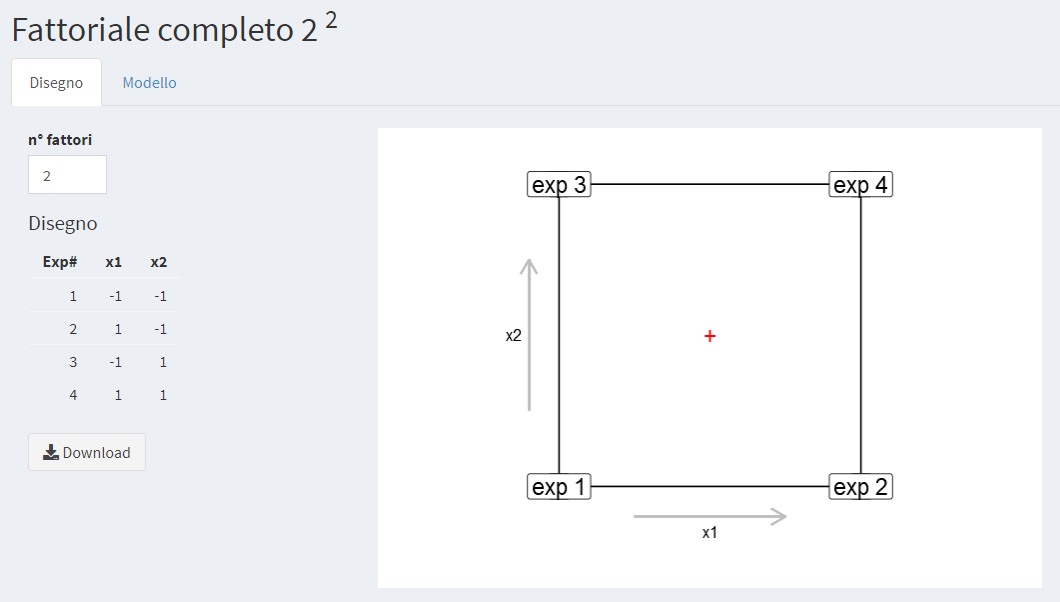
\includegraphics[width=1\linewidth]{Immagini/01_fattacompl2liv} 

}

\caption{Disegno fattoriale completo $2^2$\label{fig1}}\label{fig:unnamed-chunk-3}
\end{figure}

\begin{figure}

{\centering 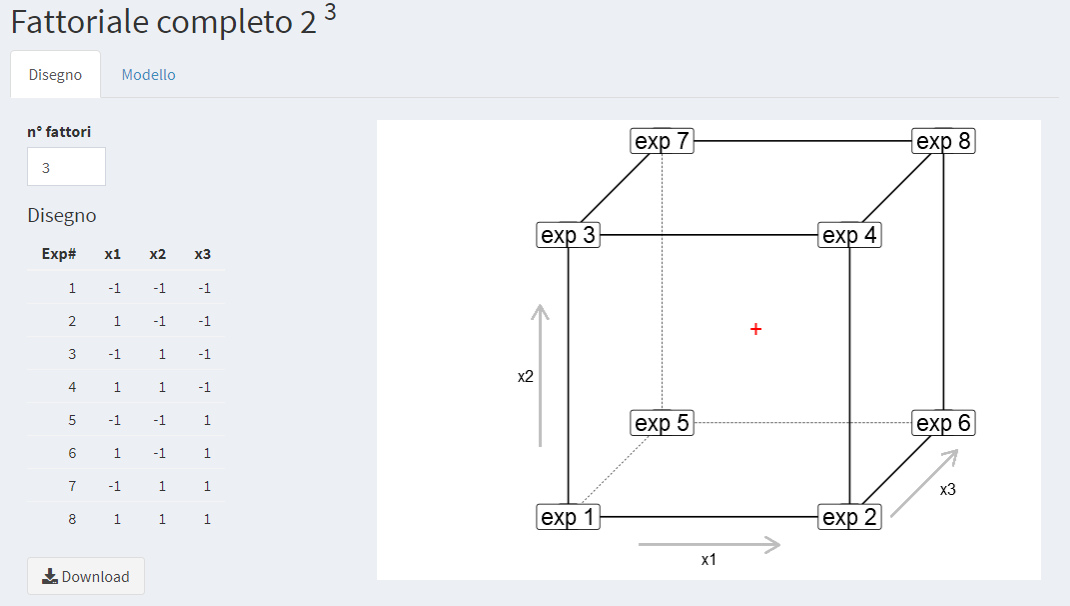
\includegraphics[width=1\linewidth]{Immagini/02_fattacompl3liv} 

}

\caption{Disegno fattoriale completo $2^3$\label{fig2}}\label{fig:unnamed-chunk-4}
\end{figure}

Consideriamo il modello lineare che tiene conto di tutti i termini lineari e di tutte le possibili interazioni
\begin{equation}\label{eq:ModDisFull}
     y_i=\beta_0+\beta_1x_{i1}+\cdots+\beta_kx_{ik}+\beta_{12}x_{i1}x_{i2}+\cdots+\beta_{1\dots k}x_{i1} \cdots x_{ik}+\epsilon_i, \qquad i=1,\dots,2^k,
\end{equation}
dove \(\epsilon_i\sim N(0,\sigma^2)\) a due a due non correlate, errore sperimentale.\newline
La matrice \(X\) del modello è data dalla matrice in \autoref{tab:MatrModDisFull}

\begin{table}[ht]
\caption{Matrice modello (\ref{eq:ModDisFull})}
\

\label{tab:MatrModDisFull}
\centering
\begin{tabular}{rrrrrrrrr}
  \hline
       \vline & $Int.$ & $X_1$ & $X_2$ & $\cdots$ &  $X_k$ & $X_1X_2$ & $\cdots$ & $X_1X_2\dots X_k$ \\
  \hline
  1 \    \vline & $1 \ \ $ & -1 \ \ & -1 \ \ & $\cdots$ & -1 \ \ &  1 \ \ \ & $\cdots$ & $(-1)^k \ \ \ $\\
  2 \    \vline & $1 \ \ $ & 1  \ \ & -1 \ \ & $\cdots$ & -1 \ \ & -1 \ \ \ & $\cdots$ & $(-1)^{k-1}$\\
  3 \    \vline & $1 \ \ $ & -1 \ \ & 1  \ \ & $\cdots$ &-1  \ \ & -1 \ \ \ & $\cdots$ & . \ \ \ \ \ \ \ \\
  4 \    \vline & $1 \ \ $ & 1  \ \ & 1  \ \ & $\cdots$ &-1  \ \ &  1 \ \ \ &  $\cdots$ & . \ \ \ \ \ \ \ \\
  . \    \vline & $1 \ \ $ & .  \ \ & .  \ \ & $\cdots$ & .  \ \ &  . \ \ \ &  $\cdots$ & . \ \ \ \ \ \ \ \\
  . \    \vline & $1 \ \ $ & .  \ \ & .  \ \ & $\cdots$ & .  \ \ &  . \ \ \ &  $\cdots$ & . \ \ \ \ \ \ \ \\
  . \    \vline & $1 \ \ $ & .  \ \ & .  \ \ & $\cdots$ & .  \ \ &  . \ \ \ &  $\cdots$ & . \ \ \ \ \ \ \ \\
  . \    \vline & $1 \ \ $ & -1 \ \ & -1 \ \ & $\cdots$ & 1  \ \ &  1 \ \ \ &  $\cdots$ & . \ \ \ \ \ \ \ \\
  . \    \vline & $1 \ \ $ & 1  \ \ & 1  \ \ & $\cdots$ & 1  \ \ & -1 \ \ \ &  $\cdots$ & . \ \ \ \ \ \ \ \\
  . \    \vline & $1 \ \ $ & -1 \ \ & -1 \ \ & $\cdots$ &  1 \ \ & -1 \ \ \ &  $\cdots$ & . \ \ \ \ \ \ \ \\
 $2^k$\  \vline & $1 \ \ $ & 1  \ \ & 1  \ \ & $\cdots$ & 1  \ \ &  1 \ \ \ &  $\cdots$ & $1$\ \ \ \ \ \ \ \ \\
   \hline

\end{tabular}
\end{table}

Poiché la matrice del modello (\ref{eq:ModDisFull}) è ortogonale, i coefficienti relativi ad ogni termine lineare forniscono esattamente l'informazione di quanto varia la risposta per uno spostamento unitario del fattore relativo, ossia \(\frac{X_{max}-X_{min}}{2}\), mantenendo gli altri parametri nulli. E' quindi 1/2 l'\textbf{effetto del parametro}, cioè la differenza tra la media dei valori delle risposte per \(X_{max}\) e la media dei valori delle risposte per \(X_{min}\).\\
Nell'esempio numerico che trattiamo più avanti, l'effetto del parametro \(X_1\) (temperatura), vedi \autoref{fig5}, è dato dalla differenza (23) tra la media (75.75) dei 4 valori della faccia \(X_1=1\) e la media (52.75) dei 4 valori della faccia \(X_1=-1\). Il coefficiente di \(X_1\), vedi \autoref{fig6}, è esattamente 1/2 l'effetto della temperatura.

Più grande in valore assoluto è il coefficiente, e maggiore è l'effetto del relativo fattore nel dominio sperimentale scelto.

Determinato il vettore \(y\) delle risposte, eseguendo i \(2^k\) esperimenti nei punti sperimentali individuati dalla matrice sperimentale in \autoref{tab:MatrDisFull}.
(\textbf{Nota importante:} per evitare effetto di autocorrelazione nell'errore nel modello gli esperimenti non vanno eseguiti nell'ordine in \autoref{tab:MatrDisFull} ma vanno mischiati casualmente)
dobbiamo stimare

\begin{itemize}
  \item $1$ coefficiente interazione $\beta_0$ (media delle $2^k$ risposte)
  \item $k$ coefficienti termini lineari $\beta_1,\cdots,\beta_k$
  \item in generale $\frac{k!}{(k-m)!m!}$ coefficienti interazioni di ordine $m$
\end{itemize}

Si noti che per il binomio di Newton si ha che
\begin{equation*}
    \sum_{m=0}^k\frac{k!}{(k-m)!m!}=2^k.
\end{equation*}
La matrice del modello (\ref{tab:MatrModDisFull}) è quindi un matrice quadrata \(2^k\)x \(2^k\) e poiché le sue colonne sono a due a due ortogonali è una matrice di Hadamard.

Dalla teoria della regressione sappiamo che uno stimatore del vettore dei parametri \(\beta\) del modello \ref{eq:ModDisFull} è dato dall'unica soluzione del sistema \(y=Xb\) (si vedano le diapositive \emph{Fattoriale completo})
\begin{equation}\label{eq:UnicaSolFull}
    b=X^{-1}y.
\end{equation}
e che
\[
Cov(b)=(X^tX)^{-1}=\frac{1}{2^k}I_k
\]
dove con \(I_k\) è indicata la matrice diagonale con valori tutti uguali a \(1\) sulla diagonale (matrice identità).

Nell'applicativo, scelto il numero di fattori compaiono automaticamente il modello e la matrice di dispersione (matrice \((X^tX)^{-1}\)) \autoref{fig3}

\begin{figure}

{\centering 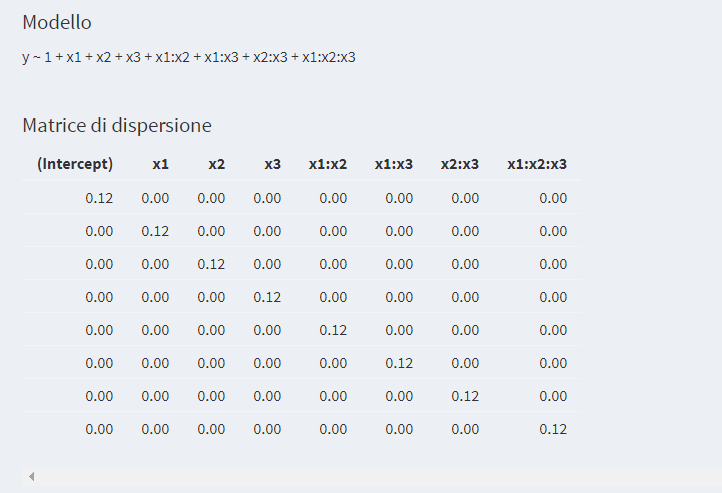
\includegraphics[width=1\linewidth]{Immagini/03_matr_disp} 

}

\caption{Modello e matrice di dispersione per un disegno fattoriale completo $2^3$\label{fig3}}\label{fig:unnamed-chunk-5}
\end{figure}

Come già osservato, la matrice di dispersione è una matrice diagonale, e questo implica che tutti i fattori sono ortogonali tra di loro
\begin{equation}\label{eq:CorrFull}
    Corr(b_i,b_j)=0, \qquad i\neq j.
\end{equation}
Il coefficiente \(\beta_j\) non cambia anche se elimino qualche fattore, o anche tutti i fattori \(X_i,\) \(i\neq j\) dal modello (la variazione dovuta da \(X_j\) sulla risposta è letta soltanto da \(\beta_j\)).

Inoltre per lo stimatore \(b=X^{-1}y\) abbiamo che
\begin{equation}\label{eq:VarFull}
    Var(b _j)=\frac{\sigma^2}{2^k}, \qquad j=1,\dots,2^k
\end{equation}

La (\ref{eq:VarFull}) ci dice la qualità dell'informazione dello stimatore \(b_j\). Ci permette inoltre di studiare la significatività statistica di \(\beta_j\) nota la varianza sperimentale \(\sigma^2\).

Essendo \(y=Xb\) un sistema di \(2^k\) equazioni (linearmente indipendenti) in \(2^k\) incognite, non abbiamo gradi di libertà, e quindi non siamo in grado di stimare \(\sigma^2\). Alla fine di questo paragrafo vedremo, se non è nota a priori la varianza \(\sigma^2\), come possiamo superare questo ostacolo.

Il valore previsto dal modello in un punto \((x_1,x_2,\dots,x_k)\) del dominio sperimentale è dato da
\[
\hat{y_0}=x_0b
\]
dove \(x_0=(1,x_1,\dots,x_1x_2,\dots,x_1x_2\cdots x_k)\) (riga della matrice del modello \autoref{tab:MatrModDisFull} corrispondente al punto \((x_1,x_2,\dots,x_k)\)). Dalla teoria sappiamo che la varianza dello stimatore \(\hat{y_0}\) è data da
\[
Var(\hat{y_0})=x_0(X^tX)^{-1}x_0^t\sigma^2
\]
La quantità \(x_0(X^tX)^{-1}x_0^t\) è chiamata \emph{Leverage} nel punto \((x_1,x_2,\dots,x_k)\).

Nell'applicativo si trova il grafico del leverage per ogni punto del dominio, \autoref{fig4}

\begin{figure}

{\centering 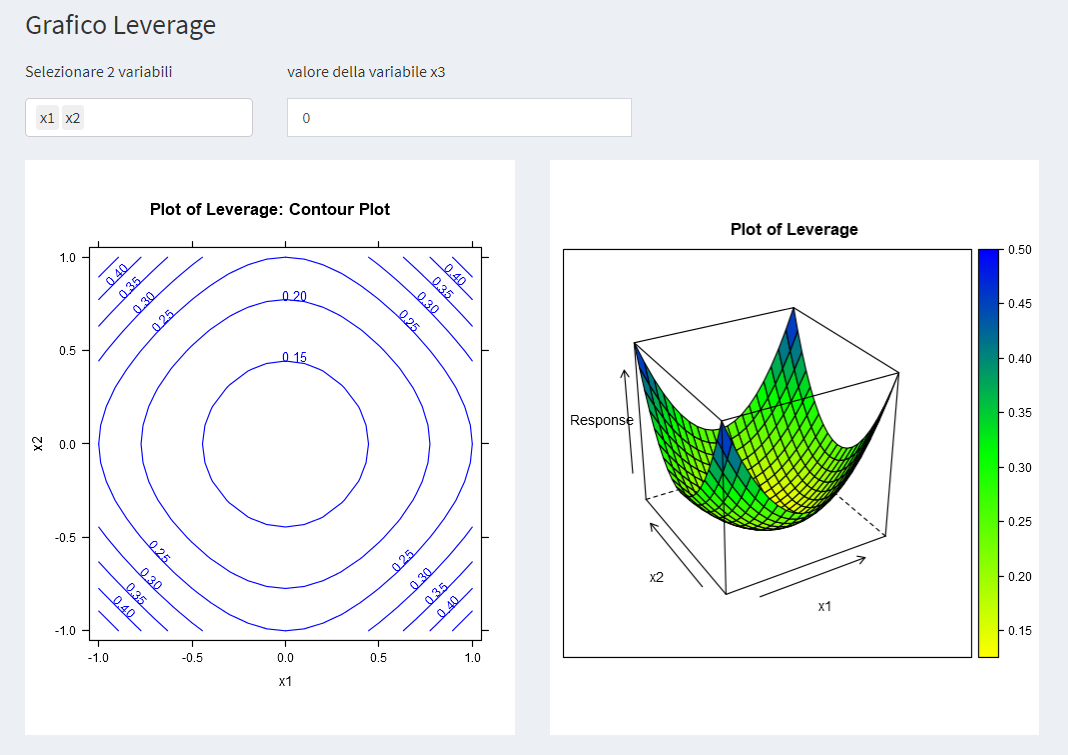
\includegraphics[width=1\linewidth]{Immagini/04_lev} 

}

\caption{Linee di livello e superficie del leverage per un disegno fattoriale completo $2^3$\label{fig4}}\label{fig:unnamed-chunk-6}
\end{figure}

La superficie di leverege ci dice com'è la qualità dell'informazione dello stimatore risposta in ogni punto del dominio sperimentale.

A questo punto è opportuno fare due osservazioni importanti:

\begin{enumerate}
\def\labelenumi{\arabic{enumi})}
\item
  il leverage non dipende dai valori delle risposte. Per questo si trova nel sotto-menù \emph{Disegno} il cui output dipende solo dal disegno.
\item
  nei punti del disegno, poiché la somma dei quadrati dei valori delle righe della matrice del modello \autoref{tab:MatrModDisFull} è \(2^k\), il valore del leverage è \(1\).\\
  Questo significa che il modello ``deve passare'' per quei punti, ma questo non deve meravigliare poiché, coma già detto, non abbiamo gradi di libertà. Per fissare le idee su questo passaggio fondamentale, siamo nello stessa situazione che conosciamo nel piano quando abbiamo solo due punti per stimare i coefficienti di una retta.
\end{enumerate}

Si noti che i \(2^k\) punti sperimentali sono i punti del dominio sperimentale di leverage massimo. Il che significa che in ognuno di questi punti l'informazione che abbiamo grazie al modello è migliore di quella che avremmo mediante un (unico) eventuale esperimento in quel punto. Ciò significa che la risposta, o meglio l'aspettativa della risposta, può essere predetta meglio (leggi con varianza minore) dal modello che da un singolo esperimento in quel punto. \newline

Consideriamo ora un esempio numerico.\\
Supponiamo ora di dover identificare le condizioni di processo di una reazione chimica. Vogliamo determinare l'influenza di 3 fattori

\begin{itemize}
\item
  \(X_1\): temperatura (°C)
\item
  \(X_2\): concentrazione del substrato (\%, p/p)
\item
  \(X_3\): tipo di catalizzatore
\end{itemize}

e delle loro interazioni sulla risposta

\begin{itemize}
\tightlist
\item
  \(Y\): resa di reazione
\end{itemize}

Dobbiamo innanzitutto scegliere il dominio sperimentale, cioè per ogni fattore dobbiamo determinare un intervallo di valori compreso tra un massimo e un minimo entro i quali studiare il fenomeno a cui siamo interessati. Abbiamo 2 fattori quantitativi, che sono la temperatura e la concentrazione del substrato, e un fattore qualitativo a 2 livelli, e questo è il tipo di catalizzatore: A o B.

\begin{table}

\caption{\label{tab:liv}Definizione dei livelli\label{livelli}}
\centering
\begin{tabular}[t]{l|l|l}
\hline
Fattori & -1 & +1\\
\hline
temperatura & 160 & 180\\
\hline
concentrazione & 20 & 40\\
\hline
catalizzatore & A & B\\
\hline
\end{tabular}
\end{table}

La matrice del disegno \autoref{tab:MatrDisFull} per 3 fattori è quella in \autoref{fig2}. Il piano degli esperimenti \autoref{esperimenti} si ottiene sostituendo a -1/+1 il valore corrispondente nella \autoref{livelli}.
\newpage

\begin{table}

\caption{\label{tab:unnamed-chunk-7}Piano degli esperimenti\label{esperimenti}}
\centering
\begin{tabular}[t]{r|r|r|l}
\hline
Exp. & Temp & Conc & Cat\\
\hline
1 & 160 & 20 & A\\
\hline
2 & 180 & 20 & A\\
\hline
3 & 160 & 40 & A\\
\hline
4 & 180 & 40 & A\\
\hline
5 & 160 & 20 & B\\
\hline
6 & 180 & 20 & B\\
\hline
7 & 160 & 40 & B\\
\hline
8 & 180 & 40 & B\\
\hline
\end{tabular}
\end{table}

Gli esperimenti sono elencati nel cosiddetto ``ordine standard''.
Per evitare di osservare effetti (errori) sistematici, gli esperimenti devono essere eseguiti in ordine casuale (random order). Alla fine degli esperimenti otteniamo i risultati in \autoref{esperimenti_r}

\begin{table}

\caption{\label{tab:unnamed-chunk-8}Piano degli esperimenti  con risposte\label{esperimenti_r}}
\centering
\begin{tabular}[t]{r|r|r|l|r}
\hline
Exp. & Temp & Conc & Cat & Resa\\
\hline
1 & 160 & 20 & A & 60\\
\hline
2 & 180 & 20 & A & 72\\
\hline
3 & 160 & 40 & A & 54\\
\hline
4 & 180 & 40 & A & 68\\
\hline
5 & 160 & 20 & B & 52\\
\hline
6 & 180 & 20 & B & 83\\
\hline
7 & 160 & 40 & B & 45\\
\hline
8 & 180 & 40 & B & 80\\
\hline
\end{tabular}
\end{table}

Per inserire le risposte nell'applicativo bisogna andare nel sotto menu \emph{Modello} e inserire le risposte nell'apposito riquadro, vedi \autoref{fig5} (da Excel basta copiare la colonna delle risposte e incollarla nel riquadro)

\begin{figure}

{\centering 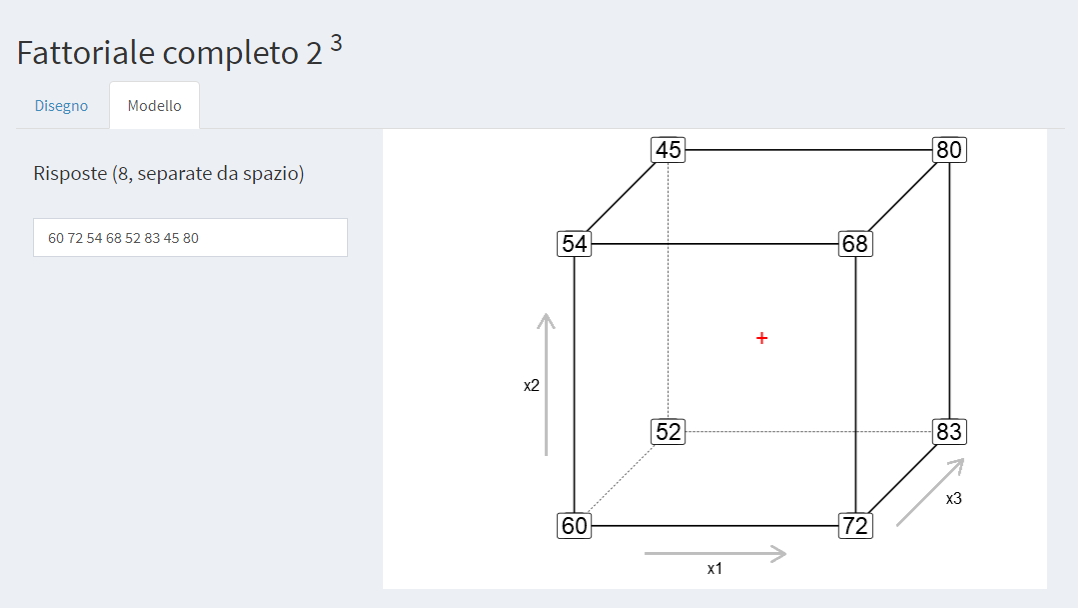
\includegraphics[width=1\linewidth]{Immagini/05_risp} 

}

\caption{Inserimento risposte nell'applicativo \label{fig5}}\label{fig:unnamed-chunk-9}
\end{figure}

Per un numero di fattori non superiore a 3 viene fornita anche una rappresentazione grafica delle risposte.

Una volta inserite le risposte, il calcolo dei coefficienti del modello è automatico e ne abbiamo anche una rappresentazione grafica, vedi \autoref{fig6}

\begin{figure}

{\centering 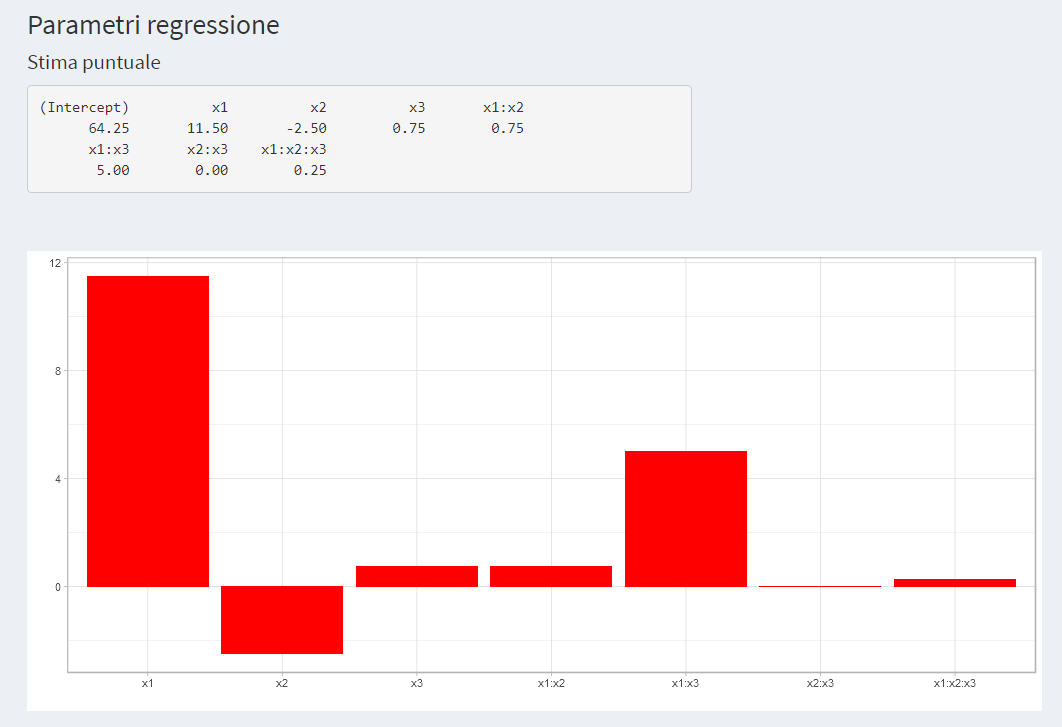
\includegraphics[width=1\linewidth]{Immagini/06_coeff} 

}

\caption{Calcolo dei coefficienti del modello \label{fig6}}\label{fig:unnamed-chunk-10}
\end{figure}

Un altro grafico riportato è il \emph{Grafico degli effetti normalizzati}, \autoref{fig7}, in cui sono rappresentati i coefficienti che contribuiscono di più nel determinare la risposta. Il grafico rappresenta la percentuale del contributo di ciascun coefficiente elevato al quadrato alla somma dei quadrati di tutti i coefficienti. I coefficienti che risultano dare un contributo in percentuale maggiore sono quelli che che influenzano maggiormente la risposta.

\begin{figure}

{\centering 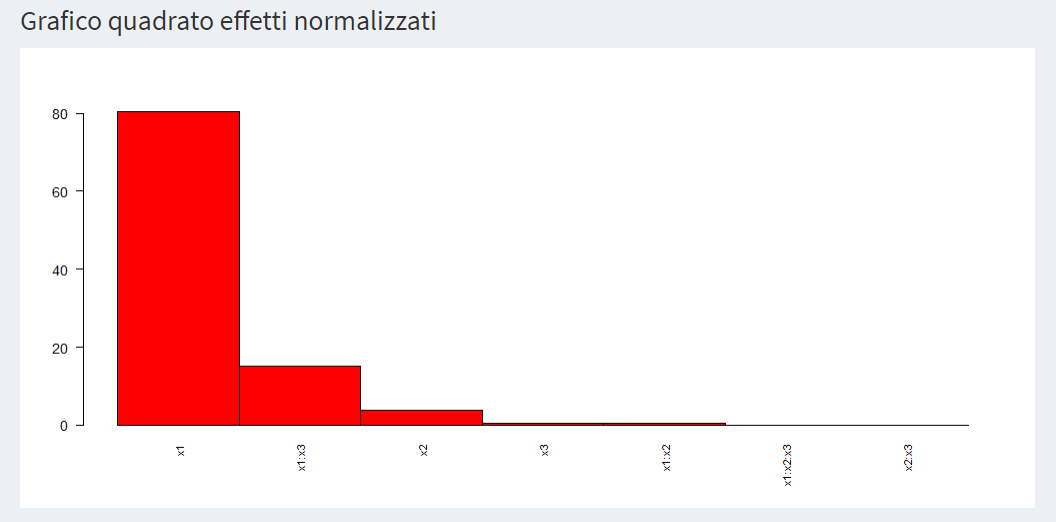
\includegraphics[width=1\linewidth]{Immagini/07_coeff_norm} 

}

\caption{Grafico degli effetti normalizzati \label{fig7}}\label{fig:unnamed-chunk-11}
\end{figure}

Dai grafici \autoref{fig6} e \autoref{fig7} risulta che i fattori che influenzano di più la risposta Resa sono la temperatura e la sua interazione con il tipo di catalizzatore.\\
In \autoref{fig8} è illustrato il grafico della superficie di risposta della Resa in funzione della temperatura e del tipo di catalizzatore, avendo fissato la concentrazione del substrato nel punto centrale del suo intervallo di variazione, vale a dire al 30\%.

\begin{figure}

{\centering 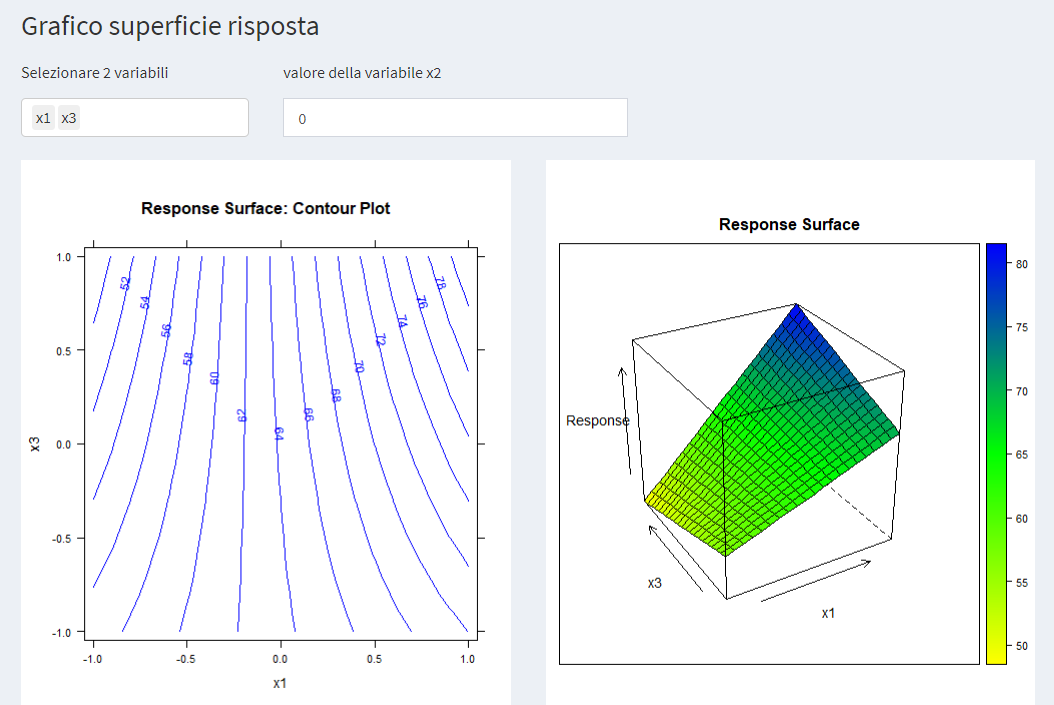
\includegraphics[width=1\linewidth]{Immagini/08_sup_risp} 

}

\caption{Grafico della superficie di risposta della Resa \label{fig8}}\label{fig:unnamed-chunk-12}
\end{figure}

Come si nota dalla \autoref{fig8} il massimo della resa si ottiene alla temperatura massima (180 °C) e usando il catalizzatore del tipo B quando il substrato è alla concentrazione del 30\%.

Circa la significatività dei coefficienti, per quanto già osservato precedentemente, non abbiamo gradi di libertà e quindi non è possibile stimare \(\sigma^2\).

Una analisi grafica della significatività dei parametri \(b_j\) può essere effettuata mediante il \emph{Normal Probability Plot}, \autoref{fig9}. Se tutti i coefficienti fossero nulli, i.e.~se fossero tutti distribuiti come una normale di media \(0\) e varianza \(\sigma^2/2^k\), essi sarebbero distribuiti come una retta. Possiamo considerare significativamente non nulli i coefficienti che si discostano dalla retta.

\begin{figure}

{\centering 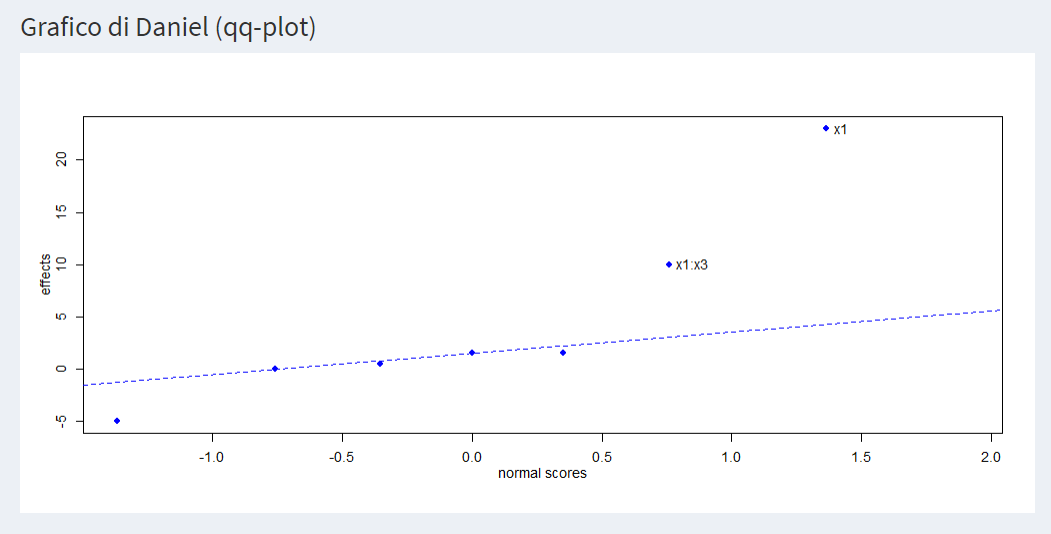
\includegraphics[width=1\linewidth]{Immagini/09_qqplot} 

}

\caption{qq-plot dei coefficienti \label{fig9}}\label{fig:unnamed-chunk-13}
\end{figure}

Dal qq-plot in \autoref{fig9} si ottiene la conferma che sono significativi (leggi: diversi da zero) la temperatura e la sua interazione con il tipo di catalizzatore.

Per convalidare il modello eseguiamo alcune misure indipendenti \(\eta_1,\dots,\eta_p\) in un punto del dominio scelto arbitrariamente. In generale si prende il centro del dominio perché è il punto in cui il leverage è minore.
Possiamo determinare \(\sigma^2\) con lo stimatore
\[
s^2=\frac{1}{p-1}\sum_{p=1}^p(\eta_i-\bar{\eta})^2.
\]
Possiamo costruire l'intervallo di confidenza della misura ``vera'' in quel punto
\[
\bar{\eta}\pm t(\alpha/2,p-1)s\sqrt{1/p}
\]
per \(\alpha\) fissato (in generale \(\alpha=95\%\)).

Nel nostro caso essendo il terzo fattore qualitativo prendiamo il punto centrale tra la temperatura e la concentrazione per il catalizzatore di tipo B, ossia il punto \((X_1,X_2,X_3)=(0,0,1)\).\\
Inserendo il valore delle misure indipendenti nell'applicativo, \autoref{fig10} otteniamo il valore medio delle misure e il relativo intervallo di confidenza al 95\%, quindi il valore della deviazione standard e dei gradi di libertà

\begin{figure}

{\centering 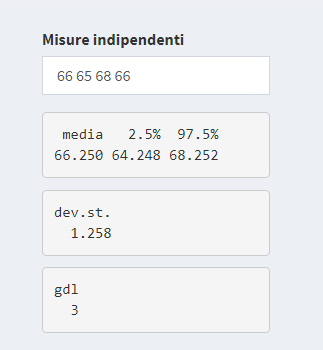
\includegraphics[width=1\linewidth]{Immagini/10_mis_ind} 

}

\caption{Misure indipendenti \label{fig10}}\label{fig:unnamed-chunk-14}
\end{figure}

Inserendo le misure indipendenti abbiamo quindi una stima di \(\sigma\) e dei gradi di libertà. Utilizzando questi valori è possibile, grazie all'\autoref{eq:VarFull}, costruire l'intervallo di confidenza dei parametri del modello. Nell'applicativo si ottengono gli estremi degli intervalli di confidenza dei parametri per alcuni valori di \(\alpha\) e i relativi \(p-value\), \autoref{fig11}

\begin{figure}

{\centering 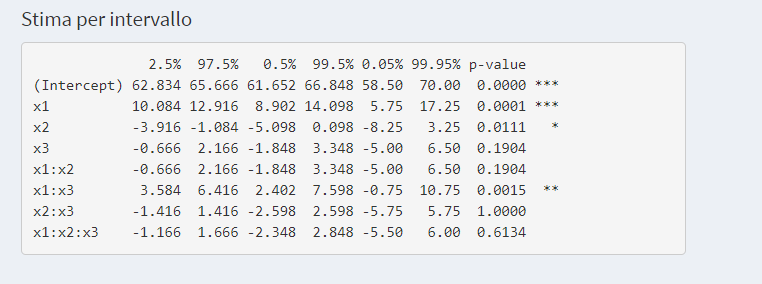
\includegraphics[width=1\linewidth]{Immagini/11_intconf} 

}

\caption{Estremi degli intervalli di confidenza dei coefficienti \label{fig11}}\label{fig:unnamed-chunk-15}
\end{figure}

Nel grafico dei parametri, l'ampiezza degli intervalli di confidenza è rapprentata con un segmento di colore verde, \autoref{fig12}

\begin{figure}

{\centering 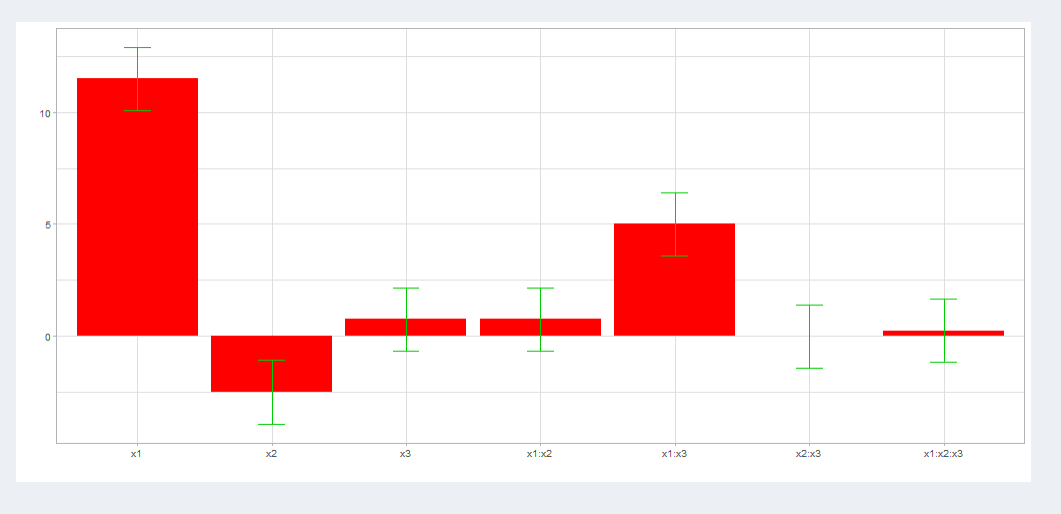
\includegraphics[width=1\linewidth]{Immagini/12_intcong_graf} 

}

\caption{Grafico dei coefficienti con estrremi degli intervalli di confidenza dei coefficienti \label{fig12}}\label{fig:unnamed-chunk-16}
\end{figure}

Per convalidare il modello bisogna quindi vedere quale è il valore previsto dal modello nel punto in cui abbiamo eseguito le misure indipendenti e verificare che non differisca significativamente dal valore ottenuto dalle misure indipendenti (ossia appartenga all'intervallo di confidenza determinato).\\
Inserendo nell'applicativo le coordinate del punto in cui sono state eseguite le misure indipendenti otteniamo la previsione del modello in quel punto e gli estremi dell'intervallo di confidenza costruiti con la stima di \(\sigma\) ottenuta, \autoref{fig13}

\begin{figure}

{\centering 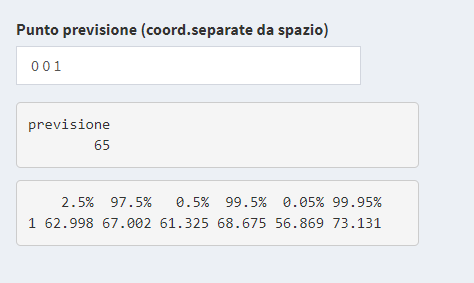
\includegraphics[width=1\linewidth]{Immagini/13_prev} 

}

\caption{Previsione del modello in un punto\label{fig13}}\label{fig:unnamed-chunk-17}
\end{figure}

Nel nostro esempio numerico il modello risulta convalidato.

  \bibliography{book.bib,packages.bib}

\end{document}
